% 10. 轧钢有两道工序:粗轧和精轧。粗轧钢坯时由于各种随机因素的影响,得到的钢材的长度呈正态分布,其均值可由轧机调整,而方差是设备精度决定的,不能改变;精轧时将粗轧得到的钢材轧成规定的长度(可以认为没有误差)。如果粗轧后的钢材长度大于规定长度,精轧时要把多出的部分轧掉,造成浪费;如果粗轧后的钢材长度已经小于规定长度,则整根报废,浪费更大。问题是已知钢材规定的长度l 和粗轧后的钢材长度的均方差sigma,求可以调整的粗轧时钢材长度的均值m,使总的浪费最小。试从以下两种目标函数中选择一个,在l=2m,sigma=20cm 条件下求均值m:
% 1)每粗轧一根钢材的浪费最小;
% 2)每得到一根规定长度钢材的浪费最小。

\subsubsection{算法设计}

\paragraph{模型建立} 由题意,钢材的规定长度为$l$,粗轧得到的钢材长度服从正态分布$N(m,\sigma^2)$,记其概率密度函数为$f(x)$,累积分布函数为$F(x)$。

对于第1个目标函数,每粗轧一根钢材的浪费长度为,
\begin{equation}
    u(m) = \int_{-\infty}^l xf(x)dx + \int_l^{+\infty} (x-l)f(x)dx = m - l(1-F(l))
\end{equation}

对于第2个目标函数,每得到一根规定长度钢材的浪费长度为,
\begin{equation}
    v(m) = \frac{u(m)}{1-F(l)} = \frac{m}{1-F(l)} - l
\end{equation}

分别求出最佳均值$m$,使得$u(m)$和$v(m)$取最小值即可。

\paragraph{算法实现} 对于累积分布函数,可采用\texttt{normcdf}命令,对于最小值求解,可采用\texttt{fminunc}命令。

\subsubsection{程序}

请参见附录\ref{sec:ex9_code}。

\subsubsection{计算结果}

为了生产出合格的钢材并减少浪费,最佳均值$m$应当在2附近,首先画出区间[2,3]中的$u(m)$和$v(m)$图像,如\Cref{fig:ex9_waste}。可以看出,最小值在$m=2.3$附近,因此将其作为初值进行求解。

\begin{figure}[H]
    \centering
    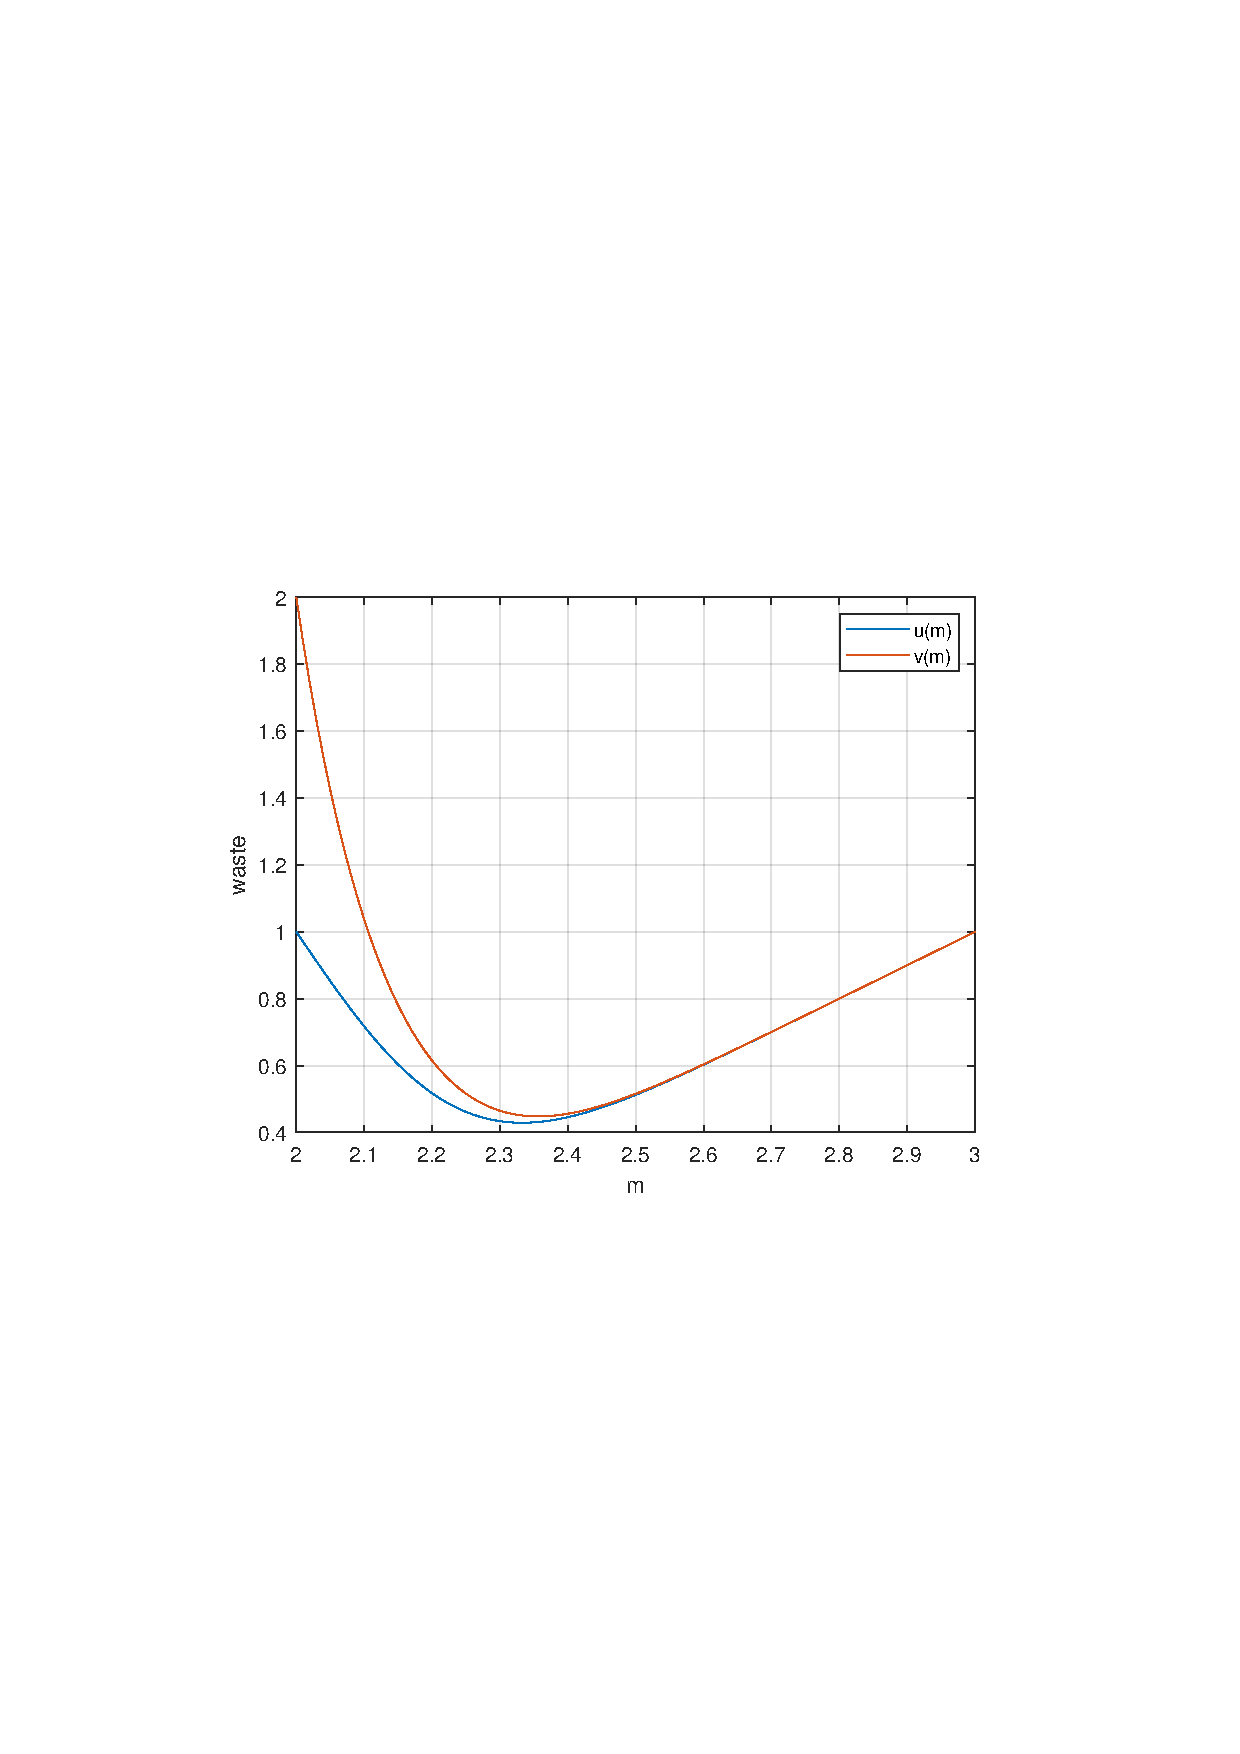
\includegraphics[width=0.8\textwidth,trim={3.09cm 9.295cm 3.09cm 9.295cm},clip]{fig/ex9_waste.pdf}
    \caption{两种目标函数的图像}
    \label{fig:ex9_waste}
\end{figure}

对于第1个目标函数,求解得到$m=2.3327$,此时浪费长度最小,为$u(m)=0.4289$。

对于第2个目标函数,求解得到$m=2.3562$,此时浪费长度最小,为$v(m)=0.4479$。

\subsubsection{结果分析}

由\Cref{fig:ex9_waste}可以看出,当$m$低于最优值时,粗轧得到钢管长度较短,导致整根报废的钢管数量较多,均摊到每根钢管的浪费长度较大;当$m$高于最优值时,粗轧得到的每根钢管长度较长,精轧时的浪费长度也较大;当$m$处于最优值时,达到了两者的平衡,此时平均浪费长度最小。

实际生产以利润为最终目标,生产利润往往与合格钢材的数量成正比,当生产每根合格钢材的浪费最小时,生产总利润最大,因此,在实际应用中,应当采用第2个目标函数。

\subsubsection{结论}

要求每粗轧一根钢材的浪费最小时,最优的粗轧钢材长度均值为2.3327米,此时平均浪费长度最小,为0.4289米。

要求每得到一根规定长度钢材的浪费最小时,最优的粗轧钢材长度均值为2.3562米,此时平均浪费长度最小,为0.4479米。
